\section{研究背景与范围}

BaZn$_2$Si$_2$O$_7$ 是 BaO--ZnO--SiO$_2$ 体系中具有可逆结构转变的硅酸盐。其低温相表现出显著的正热膨胀，加热后形成的高温相则可呈近零或负热膨胀，因而成为研究四面体链柔性和组成调控的模型体系。Lin 等通过高温 X 射线衍射（HT\nobreakdash-XRD）解析了这一相变及两种晶体结构，为后续相控制研究提供了结构基准 \cite{lin1999phase}。

本综述围绕三个问题展开：第一，BaZn$_2$Si$_2$O$_7$ 的结构和合成条件如何共同决定主相；第二，Ba\slash Sr、Zn\slash Mg\slash Co\slash Ni\slash Cu 和 Si\slash Ge 取代能够在多大范围内调节相稳定性；第三，将 Ba$_5$Y$_{12}$Zn[O(SiO$_4$)]$_8$ 视为结构类似物有哪些可核查的依据。公开数据库可确认 BaZn$_2$Si$_2$O$_7$ 的正交结构、Ba 的五配位以及 ZnO$_4$ 与 SiO$_4$ 四面体的角共享网络 \cite{available2020materials}，但本次检索未找到 Ba$_5$Y$_{12}$Zn[O(SiO$_4$)]$_8$ 可核验的原始晶体学论文。因此，全文将“直接报道”“结构相关化合物”和“结构推断”严格区分。

结构相关化合物并非仅作背景。Ba$_{1-x}$Sr$_x$Zn$_2$Si$_2$O$_7$ 的研究表明，少量 Sr 取代即可将高温结构稳定至室温，并使热膨胀系数进入负值区间 \cite{thieme2015ba1,thieme2016very}；Zn 位的异价或等价取代则进一步改变相变温度和各向异性 \cite{thieme2016new,kerstan2013bazn2si2o7}。这些结果为目标类似物的比较提供了可迁移的结构--工艺关联，但并不意味着 Ba$_5$Y$_{12}$Zn[O(SiO$_4$)]$_8$ 已被合成。

图~\ref{fig:roadmap} 给出全文的行文顺序，图~\ref{fig:taxonomy} 将结构、合成、相控制和证据边界纳入同一框架。

\begin{figure}[t]
  \centering
  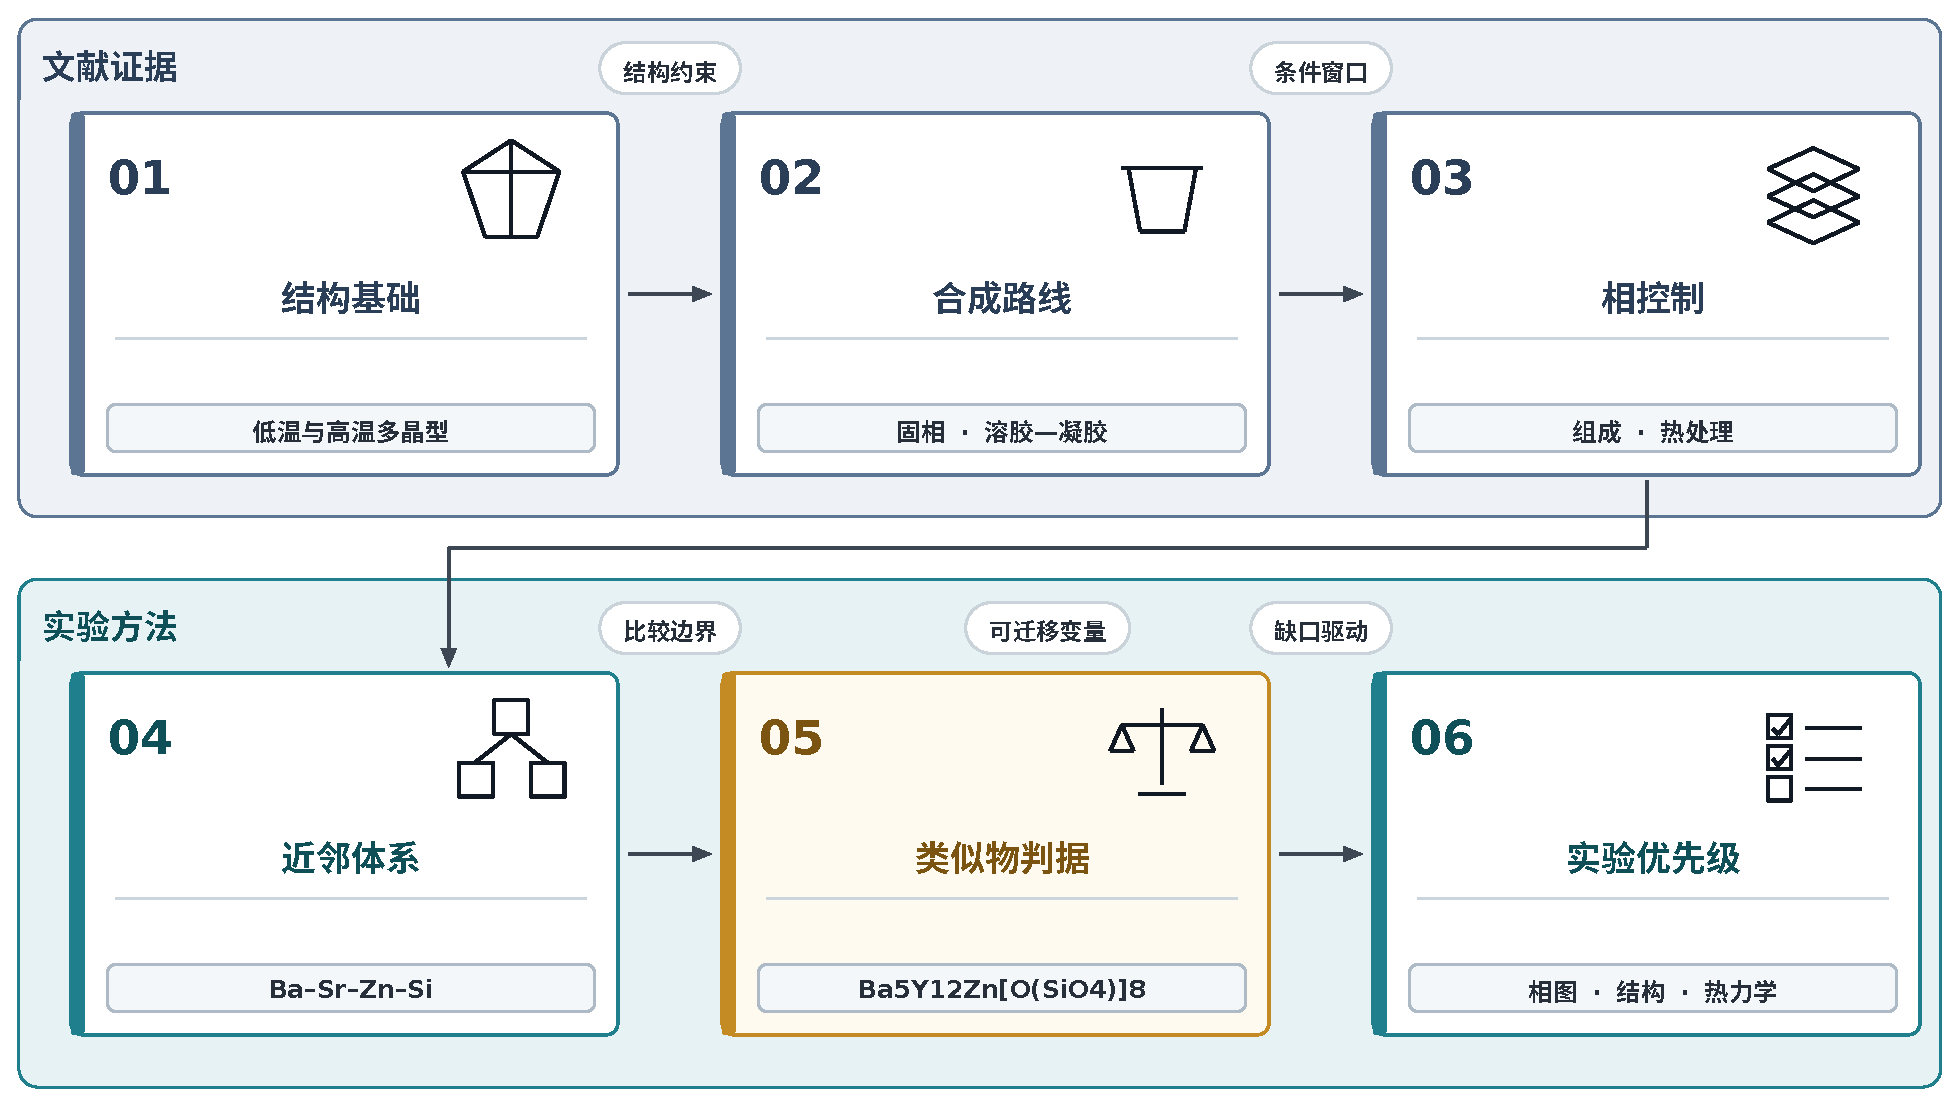
\includegraphics[width=\linewidth]{../figures/pdf/roadmap_bazn2si2o7.pdf}
  \caption{\textbf{本文的行文路线图。}箭头表示从结构事实到合成窗口、结构相关化合物规律的迁移和可证伪实验建议的推进顺序。}
  \label{fig:roadmap}
\end{figure}
